%% ------------------------------------------------------------------ %%
\chapter{Introdução}
\label{cap:introducao}

O problema de caminhos mínimos (\spp~-- \emph{shortest path problem}) é 
um dos problemas fundamentais da computação. Vem sendo estudado com 
profundidade e há uma grande quantidade de publicações a respeito do 
mesmo. Inclusive, são conhecidos várias soluções eficientes (algoritmos 
de tempo polinomial) para o problema. O \spp~é frequentemente colocado 
em prática em uma grande variedade de aplicações em diversas áreas, não 
somente em computação. Nessas aplicações geralmente se deseja realizar 
algum tipo de deslocamento ou transporte entre dois ou mais pontos 
específicos em uma rede. Tal ação deve ser executada de forma ótima em 
relação a algum critério, por exemplo o menor custo possível, ou o menor 
gasto de tempo ou o máximo de confiabilidade/segurança.

Conforme essas soluções para o \spp~foram sendo apresentadas, novas 
necessidades foram levantadas e surgiram variações do problema para 
modelar tais necessidades. Uma dessas variantes, advém do fato de que, 
na prática, muitas vezes não desejamos apenas o menor custo ou o menor 
tempo, mas desejamos otimizar uma combinação de diferentes critérios, 
por exemplo, um caminho que seja rápido e barato. Este é conhecido como 
o problema de caminhos mínimos multi-objetivo. Como não é possível 
otimizar sobre todos os critérios de uma só vez, nós escolhemos um dos 
critérios para representar a função custo, que será minimizada, e para 
os demais critérios representamos como recursos e definimos os limites 
que julgamos aceitáveis para o consumo de cada um desses recursos 
\footnote{Restrições deste tipo, onde temos o consumo de recursos em um 
  orçamento que limita a quantidade disponível destes recursos são 
chamadas de \emph{knapsack constraints} \citep{bordorfer:09}.}.  Esta 
variação é chamada de problema de caminhos mínimos com restrições por 
recursos, ou como preferimos chamar, {\bf problema de caminhos mínimos 
com recursos limitados} (\rcsp~-- \emph{resource constrained shortest 
path problem} \footnote{\citet{beasley:89} foi um dos primeiros a chamar 
  o problema desta forma, antes disso era comum utilizar apenas 
  \csp~(constrained shortest path problem). A versão com um único 
  recurso pode ser referenciada como \srcsp (\emph{single} \rcsp), ou 
  ainda como \textsc{WCSP} (\emph{weight constrained shortest path 
problem}) \citep{dumitrescu:03}.}), o qual será o objeto de estudo neste 
trabalho.

A adição de restrições por recursos no \spp, infelizmente torna o 
problema $\mathcal{NP}$-difícil, mesmo em grafos acíclicos, com 
restrições sobre um único recurso, e com todos os consumos de recursos 
positivos. Temos reduções dos famosos problemas $\mathcal{NP}$-difíceis 
\mochila~e \particao~para o nosso problema. 

Em contextos diversos são encontrados problemas de cunho teórico e 
prático que podem ser formulados como problemas de caminhos mínimos com 
recursos limitados, o que nos motivou a estudá-lo a fim de desenvolver 
um trabalho que resumisse informações suficientes para auxiliar 
pesquisadores ou desenvolvedores que tenham interesse no problema.
Nós apresentamos aqui, uma detalhada revisão bibliográfica do \rcsp, 
tendo como foco o desenvolvimento de algoritmos exatos para o caso onde 
possuímos um único recurso e a implementação e comparação dos principais 
algoritmos conhecidos, observando-os em situações práticas.

\section{Aplicações}

O problema de caminhos mínimos com recursos limitados pode ser aplicado 
em uma imensa quantidade de problemas práticos. Esta seção vai descrever 
algumas destas aplicações.

%Dentre as aplicações para o problema de caminhos mínimos com recursos 
%limitados podemos citar: transporte e comunicação, controle de frota de 
%veículos em rodovias, roteamento em redes, tratamento de redes de 
%esgoto, modelagem de cadeias de abastecimento, planejamento de 
%investimentos e avaliação de projetos, balanceamento de linhas de 
%transferência (generalização do problema de balanceamento de linhas de 
%montagem), programação e planejamento; qualidade de serviço em redes de 
%comunicação (\textsc{QoS} -- \emph{quality of service}); além de alguns 
%problemas clássicos, como \emph{matching} e variações do problema do 
%caixeiro viajante. O \rcsp~aparece ainda como subproblema em métodos de 
%geração de colunas (\cg~-- \emph{column generation}).



\subsection{Qualidade de serviço em redes de computadores}

A qualidade de serviço (\textsc{QoS} -- \emph{quality of service})
é um aspecto importante para as redes de pacotes como um todo e para as 
redes \textsc{IP} em particular. Tem um valor fundamental para o 
desempenho de determinadas aplicações fim-a-fim, como vídeo e áudio 
conferência e transferência de dados.

Existem redes de computadores que estão oferecendo garantias de 
\textsc{QoS} para diversas aplicações. Estas aplicações possuem diversos 
requisitos que precisam ser atendidos para o seu bom funcionamento.  
Como exemplo de requisitos podemos citar largura mínima de banda, tempo 
máximo de atraso e quantidade máxima de perda de pacotes. O problema em 
que estamos interessados, ou seja, serviços baseados em QoS, é 
determinar uma rota que usa os recursos da rede de forma eficiente e 
satisfaz, ao mesmo tempo, requisitos como qualidade de conexão. Este 
problema é conhecido como roteamento baseado em QoS 
\citep{aurrecoechea:98}.

\begin{figure}[h!]
  \centering
  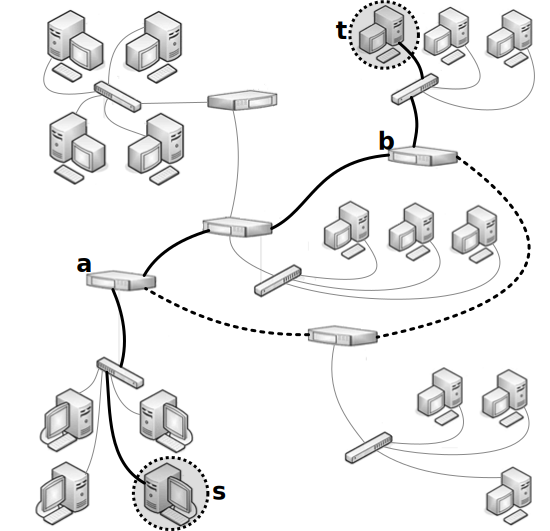
\includegraphics[scale=0.5]{figuras/pdf/qos.pdf}
  \caption[Representação de rotas em uma rede de 
  computadores]{Representação de uma rede de computadores. Os 
  seguimentos pretos e contínuos compõem uma rota entre os computadores 
  $s$ e $t$. Substituindo-se o trecho entre os roteadores $a$ e $b$ pelo 
  trecho pontilhado, temos uma outra rota que pode ser usada para a 
  comunicação entre $s$ e $t$. Dependendo das propriedades destas rotas 
  e das necessidades dos usuários, uma ou outra pode ser mais apropriada 
para o uso.}
  \label{fig:rscp_mochila}
\end{figure}

Formalizando um pouco melhor o problema, podemos representar nossa rede 
como um grafo direcionado $G = (V, A)$, onde $V$ é o
conjunto de vértices e $A$ é o conjunto de arcos. Cada arco $uv \in A$ é 
associado com um custo $c_{uv}$ e $M$ pesos não negativos  $w_{uv}^k$, 
$k=1,2,\cdots,M$ que representam a valoração dos requisitos no arco 
(ambos, pesos e custos são aditivos em um caminho).  Dada uma aplicação 
que exige $M$ requisitos com valoração máxima $R^k$ , $k = 1, 2, \cdots, 
M$, o problema é encontrar um caminho $P$ da origem $s$ até o destino 
$t$ que respeita os requisitos e que minimiza o custo total do caminho.  
Problema este que pode ser modelado da seguinte forma:

\begin{linearprogram}
\mbox{minimize}
& c(P) & = & \displaystyle\sum_{uv \in P} c_{uv} \\
\mbox{sujeito a}
&\displaystyle\sum_{uv\in P}{w_{uv}^k} &\leq& R^k & \text{para } k = 
1,\dots,M\\
\end{linearprogram}

Este problema é uma aplicação direta do problema de caminhos mínimos com 
recursos limitados. É comum, neste tipo de aplicação, querermos uma rota 
passando pelo menor número de vértices possível, neste caso a função de 
custo possui valor unitário para todos os arcos. É comum também 
existirem restrições que não são aditivas pelo caminho, mesmo com este 
tipo de restrição as soluções para o \rcsp~podem ser aplicadas, podemos 
contorná-las geralmente com algum preprocessamento ou pequenas 
alterações nos algoritmos.

\subsection{Roteamento de tráfego de veículos}

Quando precisamos nos deslocar de um ponto a outro em uma rede de 
tráfego veicular é natural nos preocuparmos com uma série de fatores a 
respeito da rota escolhida para o trajeto. Geralmente desejamos 
percorrer o caminho no menor tempo possível dentro de determinadas 
restrições, como consumo de combustível, gastos com pedágio e distância 
máxima percorrida. Outras restrições relevantes, são por exemplo, 
segurança e possibilidade de congestionamentos (essas características 
são mais subjetivas, geralmente baseadas em dados estatísticos).

Dentro deste contexto, \citet{jahn:05} propõe uma aplicação interessante 
que usa o \rcsp~como subproblema. Nesta aplicação, não se deseja 
minimizar apenas o tempo de percurso de cada usuário individualmente, o 
objetivo é minimizar o tempo total de percurso do sistema como um todo.  
Com a função objetivo da forma que foi descrito acima, é possível que 
para atingir a eficiência global, alguns usuários precisem realizar 
caminhos muito piores do que realizariam caso utilizassem uma estratégia 
egoísta. Assim, em um sistema de apoio à decisão, poderia acontecer dos 
usuários não seguirem as recomendações apresentadas. Pensando nisto, 
\citet{jahn:05} aplica uma restrição para que o caminho de cada usuário 
não seja demasiadamente pior do que o melhor caminho possível. Desta 
forma, é possível obter uma solução aceitável para cada usuário, que 
objetiva aumentar a eficiência global do sistema \footnote{Soluções onde 
  se atribui o caminho mais rápido para cada usuário sob as condições 
  correntes, são chamadas de solução \emph{user optimal} ou \emph{user 
  equilibrium}.  Soluções onde minimiza-se o tempo total do sistema, são 
chamadas de \emph{system optimal}.}.

Hoje em dia existem sistemas de informação e orientação projetados para 
auxiliar motoristas a tomarem decisões de rota. Vamos idealizar um 
sistema que pode fornecer informações como congestionamentos, bloqueios 
ou acidentes, e dar recomendações baseado nestes dados. O motorista 
cadastraria suas preferências, entraria com o seu destino e o sistema 
calcularia a rota baseado nos mapas digitais, preferências do usuário, 
especificidades do veículo (dimensões, quantidade de combustível 
disponível e consumo, por exemplo) e nas condições atuais do trânsito.  
Sistemas deste tipo poderiam ter o seguinte cenário, as condições de 
tráfego seriam obtidas através de sensores e transmitidas a uma central 
de controle de tráfego, que por sua vez, receberia (talvez do computador 
de bordo do carro) as preferências dos usuários, as características dos 
veículos, as posições atuais e seus destinos, podendo assim fazer certas 
distribuições de rotas aos motoristas.

\begin{figure}[h!]
  \centering
  \includegraphics[scale=0.5]{figuras/jpg/gps.jpg}
  \caption[Sistema de orientação para motoristas]{Exemplo de um sistema 
    de orientação para motoristas. No lado esquerdo podemos ver para uma 
    determinada região o tráfego em cada trecho (vermelho, amarelo e 
    verde representam respectivamente tráfego pesado, médio e leve). No 
    lado direito temos a representação de uma rota, começando no 
    triângulo azul (posição atual do veículo) e terminando na marcação 
com um circulo quadriculado xadrez.(Figura retirada de Google Mobile 
Blog -- 
http://googlemobile.blogspot.com.br/2011/07/live-traffic-information-for-13.html)}
  \label{fig:gps}
\end{figure}

Descrevemos todo um conjunto de restrições complexo e detalhista, porém, 
na nossa formulação levaremos em consideração apenas os níveis de 
congestionamento e um limitante superior para a degradação de um caminho 
em relação ao melhor caminho (consideramos um caminho viável apenas se 
este é mais demorado que o caminho mais rápido até um certo limite).

Representamos nossa rede rodoviária por um grafo direcionado $G = (V, 
A)$ com dois atributos em cada arco $uv \in A$: $\tau_{uv} \geq 0$ que 
representa uma estimativa do tempo de travessia quando não há 
congestionamento; e uma função $l_{uv}(x_{uv})$ ($x$ é um fluxo na rede, 
$x_{uv}$ é a parte deste fluxo correspondente ao arco $uv$) que computa 
uma estimativa do tempo de travessia do arco $uv$ considerando o fluxo 
dado\footnote{
  %TODO
  TODO -- Informações sobre a função $l$.
}.

Nós modelamos os veículos que possuem a mesma origem e destino como um 
par $k = (s, t)$, definimos $K$ como o conjunto de todos estes pares.  
Podemos representar cada $k \in K$ como $(s_k, t_k)$. Definimos a 
demanda $d_k > 0$ para cada $k \in K$ como sendo a quantidade de fluxo a 
ser roteada através de $k$ (veículos por unidade de tempo). Denotamos 
todos os caminhos para o par $k$ por $\mathcal{P}_k = \{P \mid P \mbox{ 
é um caminho de } s_k \mbox{ até } t_k \}$, e o conjunto completo de 
caminhos por $\mathcal{P} = \cup_{k \in K}{\mathcal{P}_k}$. Para um 
caminho $P \in \mathcal{P}$, o tempo para percorrermos $P$, dado um 
fluxo $x$ representando o estado atual da rede, é $l_P(x) = \sum_{uv \in 
P}{l_{uv}(x_{uv})}$, o tempo estimado de percurso sem considerar 
congestionamento é $\tau_P = \sum_{uv \in P}{\tau_{uv}}$.

Definimos um fator de tolerância $\varphi \geq 1$. Através deste fator, 
assumimos que para um caminho $P \in \mathcal{P}_k$ ser viável, $\tau_P 
\leq \varphi T_k$, onde $T_k = \min_{P \in {\cal P}_k}{\tau_P}$ é o 
menor tempo possível para se partir de $s_k$ e chegar a $t_k$ 
desconsiderando-se o fluxo na rede.  Assim podemos denotar 
$\mathcal{P}_k^\varphi$ como o conjunto de todos os caminhos viáveis que 
partem de $s_k$ e terminam em $t_k$, e $\mathcal{P}^\varphi = \cup_{k 
\in K}{\mathcal{P}_k^\varphi}$ como sendo o conjunto de todos os 
caminhos viáveis para os pares em $K$.

O sistema ótimo com restrições (\textsc{CSO} -- \emph{constrained system 
optimum}) proposto, pode ser modelado como o seguinte fluxo múltiplo de 
custo mínimo (\emph{min-cost multi-commodity flow}):

\begin{linearprogram}
\mbox{minimize}
& C(x) & = & \displaystyle\sum_{uv \in A} l_{uv}(x_{uv}) \cdot x_{uv} \\
\mbox{sujeito a}
&\displaystyle\sum_{P \in \mathcal{P}_k^\varphi}{x_P} &=& d_k & 
\text{para } k \in K\\
&\displaystyle\sum_{P \in \mathcal{P}^\varphi \mid uv \in P}{x_P} &=& 
x_{uv} & \text{para } uv \in A\\
       &x_P &\geq& 0 & \text{para } P \in \mathcal{P}^\varphi\\
\end{linearprogram}

\citet{jahn:05} usa um algoritmo de geração de colunas para resolver o 
problema \textsc{CSO} (para uma descrição do método ver \citet{frank:56} 
e \citet{leblanc:85}). Neste algoritmo, surge como sub-problema computar 
um caminho ótimo em $\mathcal{P}_k^\varphi$ que é precisamente o \rcsp:  
Neste caso, cada arco $uv \in A$ tem dois parâmetros, o tempo de 
travessia $l_{uv}$ e o comprimento $\tau_{uv}$.  Dado um par $(s, t)$, o 
objetivo é computar um caminho mais rápido de $s$ a $t$ cujo tamanho não 
excede a um dado limite $T$. Ou seja, o problema é $$ \min \{l_P \mid P 
\mbox{ é uma caminho de } s \mbox{ até } t \mbox{ e } \tau_p \leq T 
\}\mbox{,}$$ onde $ l_{P} = \sum_{uv \in P}l_a$ e $\tau_P = \sum_{uv \in 
P}\tau_{uv}$.

\subsection{Compressão de imagens (aproximação de curvas)}

Uma curva/função é linear por partes (\emph{piecewise linear curve}) se 
pudermos subdividi-la em intervalos que são lineares.  Este tipo de 
curva/função é frequentemente usado para aproximar funções complexas ou 
objetos geométricos.

\begin{figure}[!ht]
  \centering
  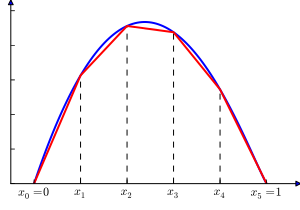
\includegraphics[scale=0.7]{figuras/pdf/funcao_linear_por_partes.pdf}
  \caption[Exemplo de uma função linear por partes]{Exemplo de uma 
    função linear por partes. A função em azul é uma função não linear, 
    e a função em vermelho é uma aproximação da primeira que atende a 
  nossa definição de curva linear por partes.}
  \label{fig:gps}
\end{figure}

O uso dessas curvas é muito comum em áreas como computação gráfica, 
programação matemática, processamento de imagens e cartografia. Curvas 
lineares por parte são populares porque são fácil de se criar e 
manipular, além de fornecer, em geral, uma aproximação suficientemente 
boa para os problemas estudados.

Aplicações nas áreas citadas no parágrafo anterior, frequentemente 
incluem uma enorme quantidade de dados (as curvas em geral possuem uma 
grande quantidade de partes ou pontos de quebra). Isto causa 
dificuldades, por exemplo, com o espaço de armazenamento, taxa de 
transmissão ou tempo gasto para renderizar a curva em um dispositivo 
gráfico. Isto naturalmente nos faz pensar no problema de 
redução/compressão de dados, onde nós queremos determinar uma nova curva 
linear por partes que é tão aproximada quando possível da original, mas 
tem um número menor de pontos de quebra.

\citet{dahl:96, nygaard:98} estudaram este problema e mostraram como ele 
poderia ser modelado como um problema de caminhos mínimos com recursos 
limitados: Os pontos de quebra $v_1, v_2, \cdots, v_{n-1}, v_n$ são os 
vértices do grafo $G = (V, A)$ e para todo para $1 \leq i \leq j \leq n$ 
nós temos um arco $v_iv_j$. O custo de um arco $c_{uv}$ é o erro 
introduzido na aproximação por tomar o ``atalho'' indo direto de $u$ 
para $v$ ao invés da curva original\footnote{Existem diversos tipos de 
métricas que podem ser usadas para calcular este erro.}. O recurso de 
uma aresta $r_{uv}$ é $1$ para $uv \in A$.  Agora, nós podemos computar 
a melhor aproximação usando no máximo $k$ pontos de quebra 
\footnote{Alternativamente, nós podemos limitar o erro de aproximação e 
computar o menor número de pontos de quebra.}.

\begin{figure}[!ht]
  \centering
  \includegraphics[scale=1]{figuras/pdf/curva.pdf}
  \includegraphics[scale=1]{figuras/pdf/curva_aproximada.pdf}
  \caption[Exemplo de uma curva e sua aproximação.]{
    Exemplo de uma curva e sua aproximação. A curva original possui $90$ 
  pontos, enquanto a sua aproximação possui $15$ pontos.}
  \label{fig:gps}
\end{figure}



\section{Objetivos}

Os principais objetivos deste trabalho, de forma sucinta são:
\begin{itemize}
  \item levantar um conjunto de referências bibliográficas relevantes, 
    cobrindo o máximo possível de variações e aplicações do problema;
\item apresentar o \rcsp~e suas diversas abordagens com uma notação 
  padronizada;
\item implementar um subconjunto dos principais algoritmos conhecidos;
\item avaliar o desempenho prático dos algoritmos implementados.
\end{itemize}

\section{Preliminares}

Para o perfeito entendimento do conteúdo desde trabalho devemos 
salientar a necessidade de conhecimento prévio em alguns assuntos que 
enumeraremos a seguir. A maioria dos estudantes de computação deve estar 
familiarizado com os conceitos, mas faremos indicações de publicações 
que definem e usam notações próximas da que estamos utilizando. 

Um conhecimento prévio dos seguintes assuntos é recomendado:

\begin{itemize}
\item Teoria dos Grafos
\item Algoritmos em Grafos
\item Fluxo em Redes
\item Programação Linear
\item Programação Inteira
\item Relaxação Lagrangiana
\item Algoritmos de Aproximação
\item Complexidade Computacional
\end{itemize}

%Para uma descrição resumida, em um só lugar, de todos os pontos acima 
%podemos indicar a seguintes teses de doutorado que abordam o nosso 
%problema: \citet{zhu:05}, \citet{ziegelmann:01}, \citet{garcia:09}. Os 
%autores abordaram o problema de uma forma extensiva e escreveram 
%preliminares interessantes.
%\citet{pf:proglin} e 

No que se trata da parte de teoria dos grafos, fluxo em redes e 
algoritmos em grafos, seguimos de perto a nomenclatura e conceitos 
definidos em \citet{pf:fluxos}. Um livro muito completo em relação aos 
conceitos de programação linear e relaxação que fazemos questão de 
indicar é o \citet{wolsey1998integer}. \citet{Carvalhoetal01} fala sobre 
algoritmos de aproximação, e é uma ótima referencia sobre o assunto.
Por fim temos o livro \citet{clrs:introalg-2001} que pode ser usado para 
o estudo de complexidade computacional.

\section{Organização}

O trabalho é organizado da seguinte forma.

O Capítulo \ref{cap:introducao} -- \nameref{cap:introducao}, apresenta 
uma visão geral do problema e da dissertação. Apresentamos textualmente 
uma definição do \rcsp, alem de citar informações sobre complexidade e 
descrever alguns problemas interessantes aos quais o \rcsp~pode ser 
aplicado. Enumeramos também os tópicos relevantes para o entendimento do 
nosso trabalho fazendo referência a textos que podem ajudar os leitores 
a adquirir tais conhecimentos. Discorremos um pouco também a respeito do 
foco e objetivos deste trabalho.

O Capítulo \ref{cap:spp} -- \nameref{cap:spp}, trás uma descrição do 
problema de caminhos mínimos clássicos, problema este que deu origem ao 
\rcsp. Alem da descrição apresentamos algoritmos eficientes para o 
problema, e também definimos alguns conceitos importantes, usados no 
decorrer da dissertação.

No Capítulo \ref{cap:rcsp} -- \nameref{cap:rcsp}, definimos formalmente 
o problema de caminhos mínimos com recursos limitados, que é o foco 
deste trabalho. Apresentamos um breve histórico listando as principais 
soluções conhecidas para o problema. Expomos também uma prova que mostra 
que o \rcsp~é um problema $\mathcal{NP}$-difícil. Por fim descrevemos 
alguns algoritmos relevantes que despertaram nosso interesse.

O Capítulo \ref{cap:experimentos} -- \nameref{cap:experimentos}, expõe 
estatísticas e percepções a respeito dos experimentos realizados com os 
algoritmos implementados.

%Por fim, no Capítulo \ref{cap:conclusao} -- \nameref{cap:conclusao},
%apresentamos as considerações finais sobre o trabalho e sugerimos 
%possíveis trabalhos futuros que poderiam dar continuidade aos estudos 
%aqui realizados.
